\documentclass[largefonts,landscape]{sciposter}

\usepackage{pstricks}
\usepackage{newcent}
\usepackage{courier}
%\usepackage{xcolor}
\usepackage[pdftex]{graphicx}
\usepackage{multirow,array}
\usepackage{amsmath,amsthm,amssymb}
\usepackage{algorithmic}
\usepackage{fancybox}
\usepackage{multicol}
\usepackage{natbib}

\definecolor{mainCol}{rgb}{0.878,0.707,0.769} %% background color
\definecolor{SectionCol}{rgb}{0.1,0.1,0.5}    %% section heading color
\definecolor{BoxCol}{rgb}{0.433,0.769,0.804}	      %% algorithm box color

\newtheorem*{theorem}{Theorem}
\newtheorem*{definition}{Definition}
\newtheorem*{conjecture}{Conjecture}

\newcommand{\R}{\mathbb{R}}
\newcommand{\x}{\mathbf{x}}
\newcommand{\w}{\mathbf{w}}
\newcommand{\ud}{\mathrm{d}}

\DeclareMathOperator*{\argmin}{argmin}

\begin{document}

\renewcommand{\thefootnote}{\fnsymbol{footnote}}
\renewcommand{\footlogo}{Typeset by pdf\LaTeX}


\title{Scale-Free and Parameter-Free Online Learning}
\author{Francesco Orabona\footnotemark[1], D\'avid P\'al\footnotemark[2]}
\institute{%
\footnotemark[1] University of Stony Brook, New York\\
\footnotemark[2] Yahoo Research, New York, NY}

\date{November 9, 2016}

\leftlogo[1.2]{uwaterloo-uw}
\rightlogo[1]{uwaterloo-cs}
\conference{Theoretical Foundations for Learning from Easy Data, November 7-11, Lorentz Center, University of Leiden, Leiden, Netherlands}

\maketitle

\setlength{\parindent}{2em}

\setlength{\columnsep}{6cm}
\begin{multicols}{3}

\section*{Introduction}

\PARstart{A}{ basic assumption} in unsupervised and semi-supervised learning
is that data points coming from different classes are separated by regions
of ``low density''. (E.g. clustering algorithms or transductive SVMs.)

\begin{center}
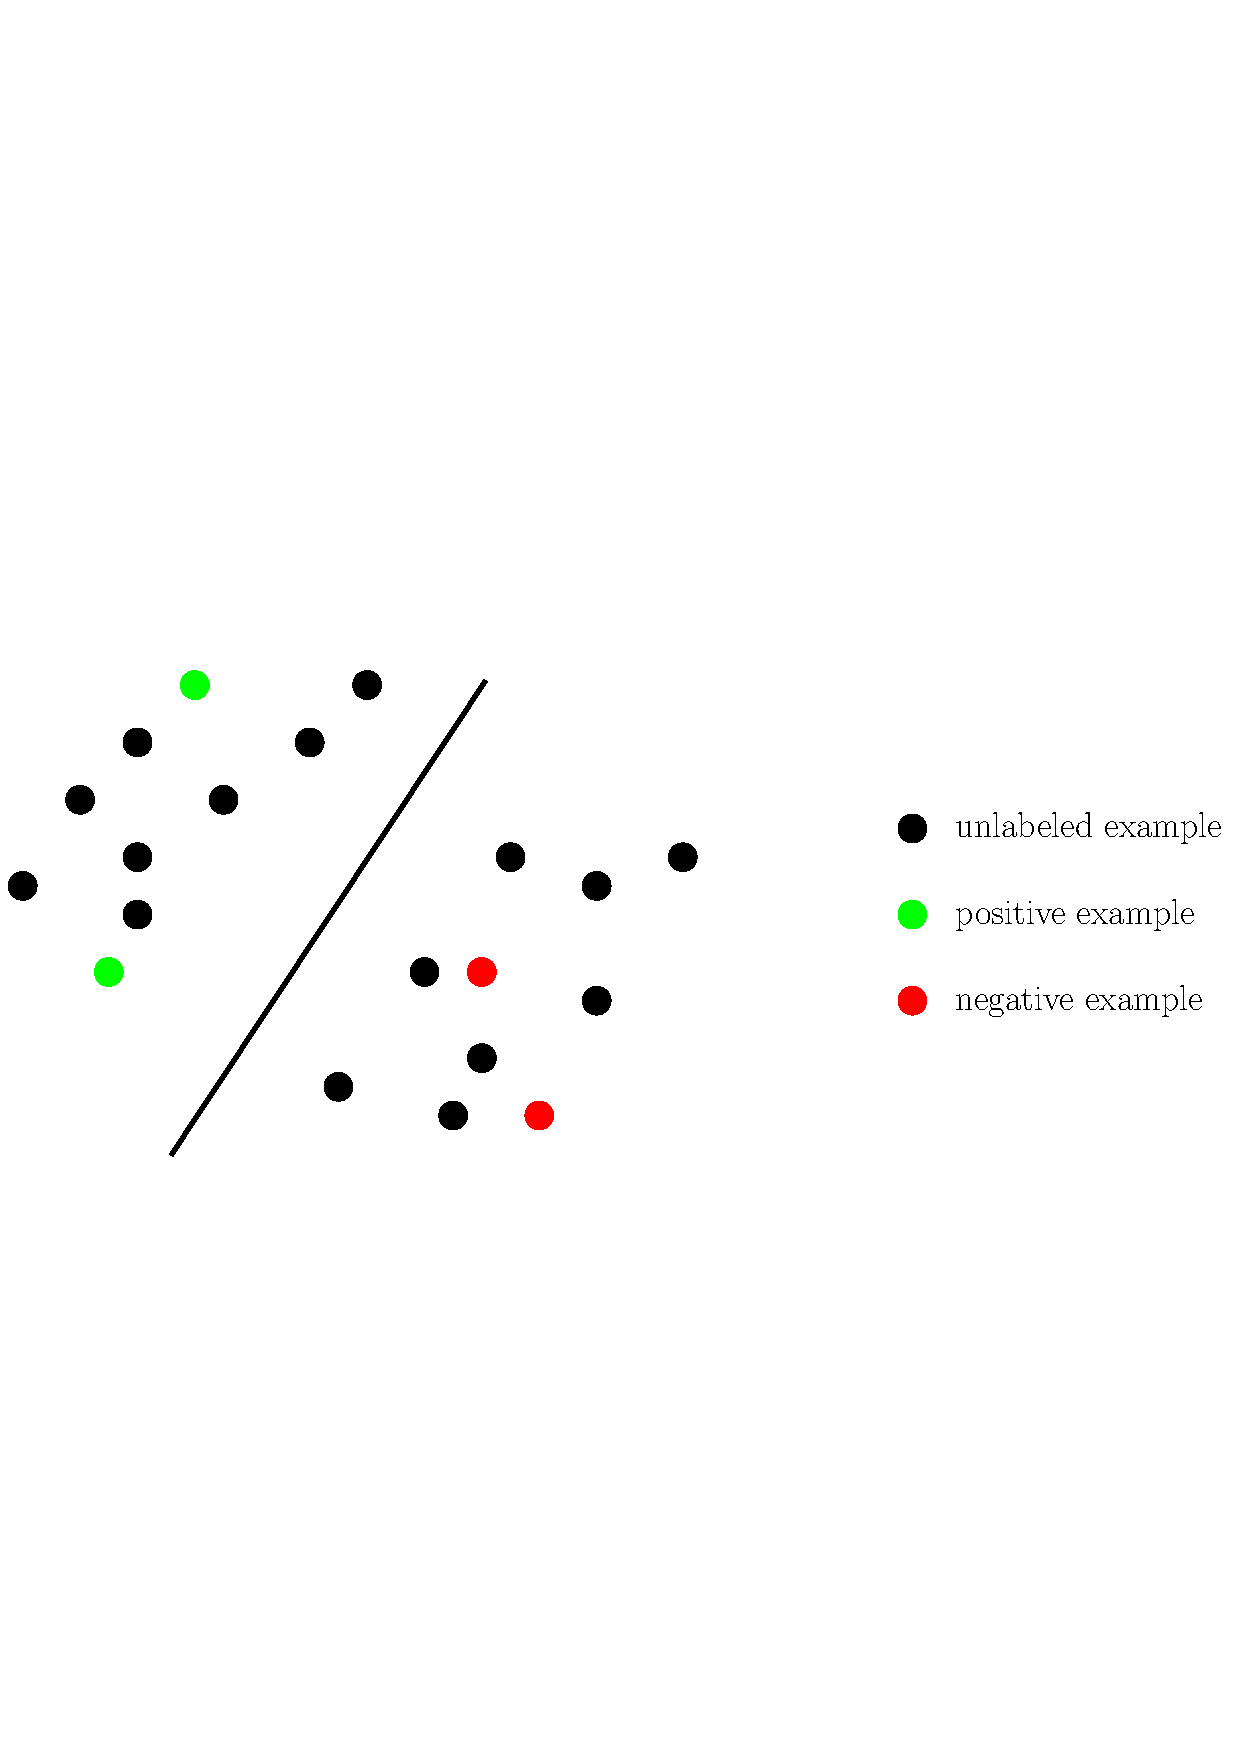
\includegraphics[scale=1.5]{tsvm}
\end{center}

Consider only two classes. Given an i.i.d. sample, how hard is to find a linear
separator of low density?

\begin{center}
%\noindent
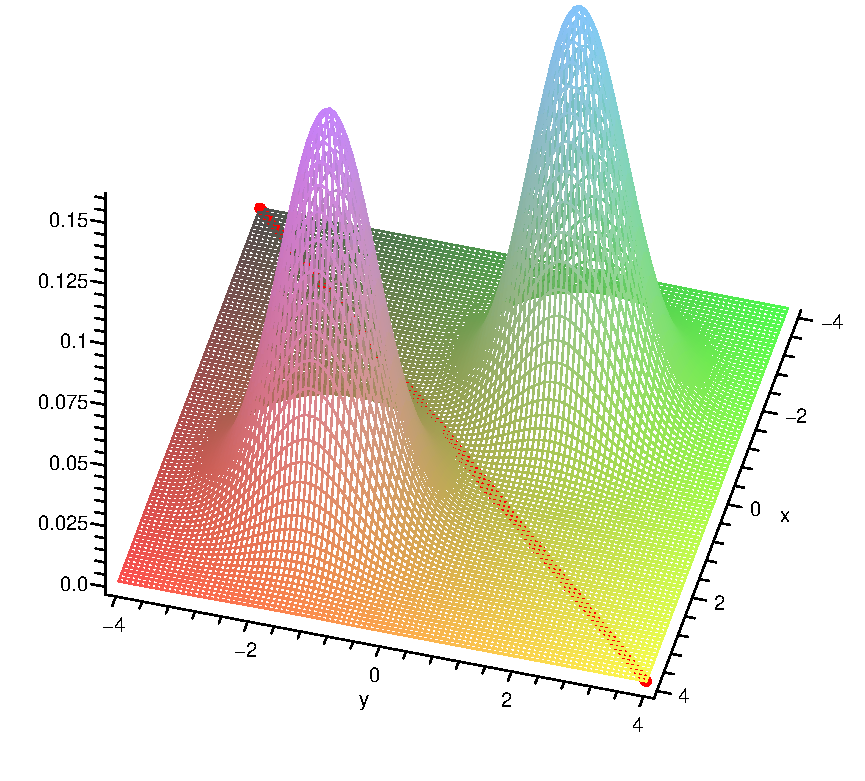
\includegraphics[width=33cm]{3dplot}
\end{center}

The above plot shows a mixture of two spherical Gaussian distributions with the same variance variance.
The line in the $xy$-plane is the separator of lowest density.

\columnbreak

\section*{The Formal Model}

\PARstart{S}{uppose} that (unlabeled) data $S=(\x_1, \x_2, \dots, \x_m)$ are sampled i.i.d. from a probability measure $\mu$ over $\R^d$
with a \emph{continuous} probability density $f:\R^d \to \R_0^+$. Find the normal $\w \in \R^d$ of a hyperplane $\w^T \x = 0$
such that the integral of the density
$$
\overline{f}(\w) \ \stackrel{\text{def}}{=} \int_{\{ \x ~:~ \w^T \x = 0 \}} \displaylimits f(x) \ \ud x
$$
\emph{on} the hyperplane is as small as possible.

Assume that $\w^*$ and $-\w^*$ are the ``unique'' minimizers of $\overline{f}$.
Can we design a learning algorithm $L:S \mapsto \w$ which is \emph{consistent} i.e. 
$$
L(S) \to \w^*  \qquad \text{in probability?}
$$
To measure the closeness between $L(S)$ and $\w^*$ we consider three metrics.

\begin{definition}
Let $\w, \w' \in \R^d$ be two unit length normal vectors. We define
\begin{align*}
& \text{1.} \quad D_E(\w,\w')  = 1-\left| \w^T \w' \right| \\
& \text{2.} \quad D_{f}(\w,\w') = \left| \overline{f}(\w') - \overline{f}(\w) \right| \\
& \text{3.} \quad D_{\mu}(\w,\w') = \min \left\{ \mu(h^+(\w) \Delta h^+(\w')), \ \mu(h^-(\w) \Delta h^+(\w')) \right\}
\end{align*}
where
$
h^+(\w) = \{ \x ~:~ \w^T \x > 0 \} \quad \text{and} \quad h^-(\w) = \{ \x ~:~ \w^T \x < 0 \} \; .
$
\end{definition}

\begin{center}
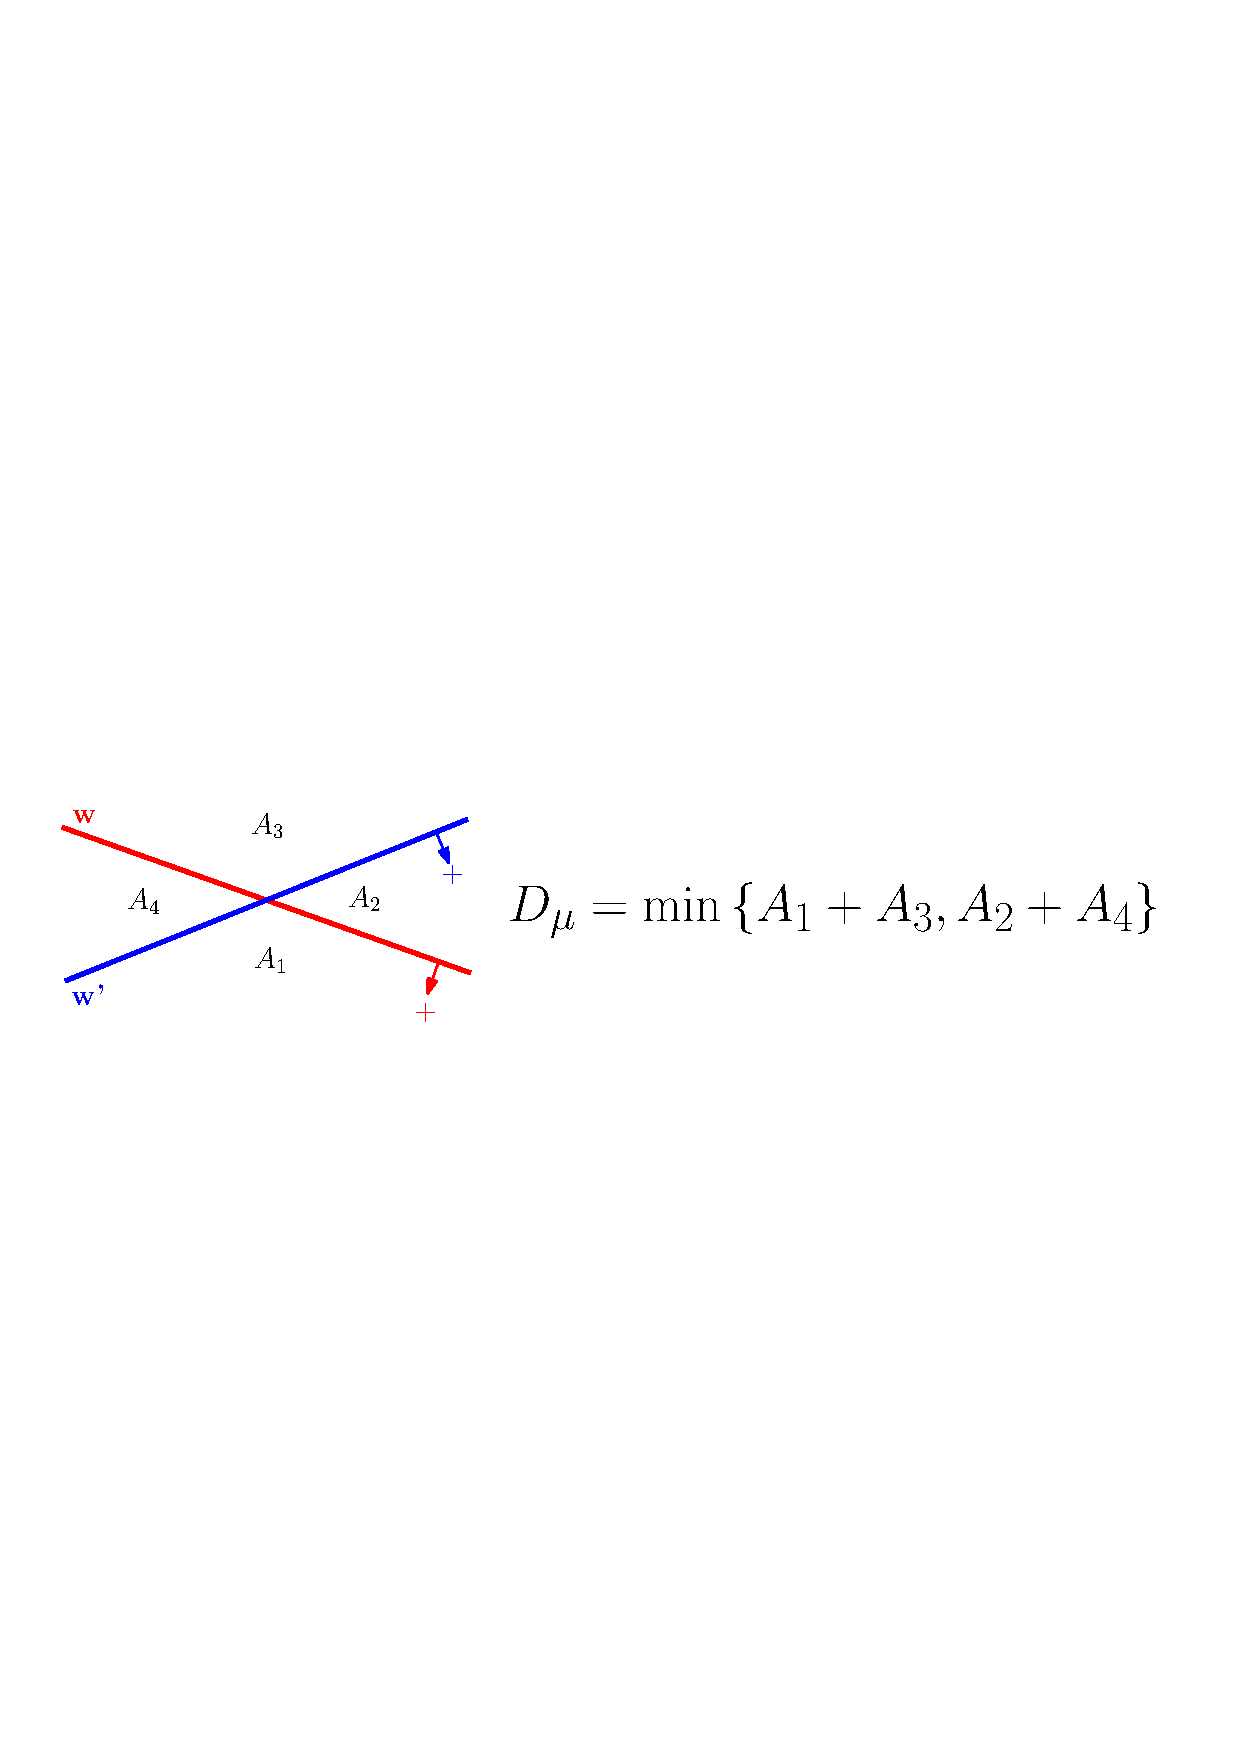
\includegraphics[scale=1.7]{two-hyperplanes}
\end{center}

\section*{The Bucketing Algorithm}

\noindent For a unit vector $\w$ and margin $\gamma > 0$ let
$$
h_\gamma(\w) = \left\{ \x \in \R^d ~:~ |\w^T \x| \le \gamma \right\} \; .
$$

\setlength{\fboxrule}{3pt}
\setlength{\fboxsep}{3pt}

\begin{center}
\colorbox[rgb]{0.980,0.820,0.199}{\fbox{
\begin{minipage}{0.25\textwidth}
\begin{algorithmic}
\STATE{\textbf{Input:} sample $S=\{\x_1, \x_2, \dots, \x_m\}$, margin $\gamma > 0$}
\vspace{0.5cm}
\STATE{Find a unit vector $\w$ with minimum $|S \cap h_\gamma(\w)|$}
\end{algorithmic}
\end{minipage}
}}
\end{center}

\vspace{0.8cm}

\begin{theorem}
The Bucketing Algorithm is consistent if $\gamma$, as a function of $m$, approaches $0$
at rate $\gamma \in \omega(1/\sqrt{m})$
\end{theorem}

\noindent For example, the choice $\gamma = 1/\sqrt[3]{m}$ makes the algorithm consistent.

\columnbreak

\section*{Hard Margin Algorithm}

\setlength{\fboxrule}{3pt}
\setlength{\fboxsep}{3pt}

\begin{center}
\colorbox[rgb]{0.980,0.820,0.199}{\fbox{
\begin{minipage}{0.25\textwidth}
\begin{algorithmic}
\STATE{\textbf{Input:} sample $S=\{\x_1, \x_2, \dots, \x_m\}$}
\vspace{0.5cm}
\STATE{Find $\w$ and $\gamma$ such that $S \cap h_\gamma(\w) = \emptyset$ maximizing $\gamma$}
\end{algorithmic}
\end{minipage}
}}
\end{center}

\vspace{0.8cm}

\begin{conjecture}
The Hard Margin Algorithm is consistent.
\end{conjecture}

\vspace{0.8cm}

\PARstart{C}{onsider} a related 1D problem: Given an i.i.d. sample $S = \{x_1, x_2, \dots, x_m\}$ from a continuous density function $f:[0,1] \to \R_0^+$
find $x^* = \argmin_{x \in [0,1]} f(x)$. The following is 1D analogue of the Hard Margin Algorithm:

\setlength{\fboxrule}{3pt}
\setlength{\fboxsep}{3pt}

\begin{center}
\colorbox[rgb]{0.980,0.820,0.199}{\fbox{
\begin{minipage}{0.25\textwidth}
\begin{algorithmic}
\STATE{\textbf{Input:} sample $S=\{x_1, x_2, \dots, x_m\}$}
\vspace{0.5cm}
\STATE{Sort $0 < x_1 < x_2 < \dots < x_m < 1$}
\STATE{(Define $x_0 = 0$ and $x_{m+1} = 1$)}
\STATE{Find $i \in \{0,1,2, \dots, m\}$ with maximum $x_{i+1} - x_i$}
\STATE{Output $(x_i + x_{i+1})/2$ (i.e. mid-point of the largest gap)}
\end{algorithmic}
\end{minipage}
}}
\end{center}

\vspace{0.8cm}

\begin{theorem}
The 1D Hard Margin Algorithm is consistent.
\end{theorem}


\section*{Impossibility of Uniform Convergence}

What is the rate of convergence $L(S) \to \w^*$ (in any of the three metrics)?
Can we guarantee a speed of convergence independent of $\mu$? No.

\begin{theorem}
For any learning algorithm $L$ and any sample size $m$ any there exists a continuous density $f:[0,1] \to \R_0^+$ such that
$$
\Pr_{S \sim f^m} \left[ D(L(S), x^*) \ge 1/4  \right] \ge 1/4
$$
where $D$ is any of the three metrics.
\end{theorem}

\begin{center}
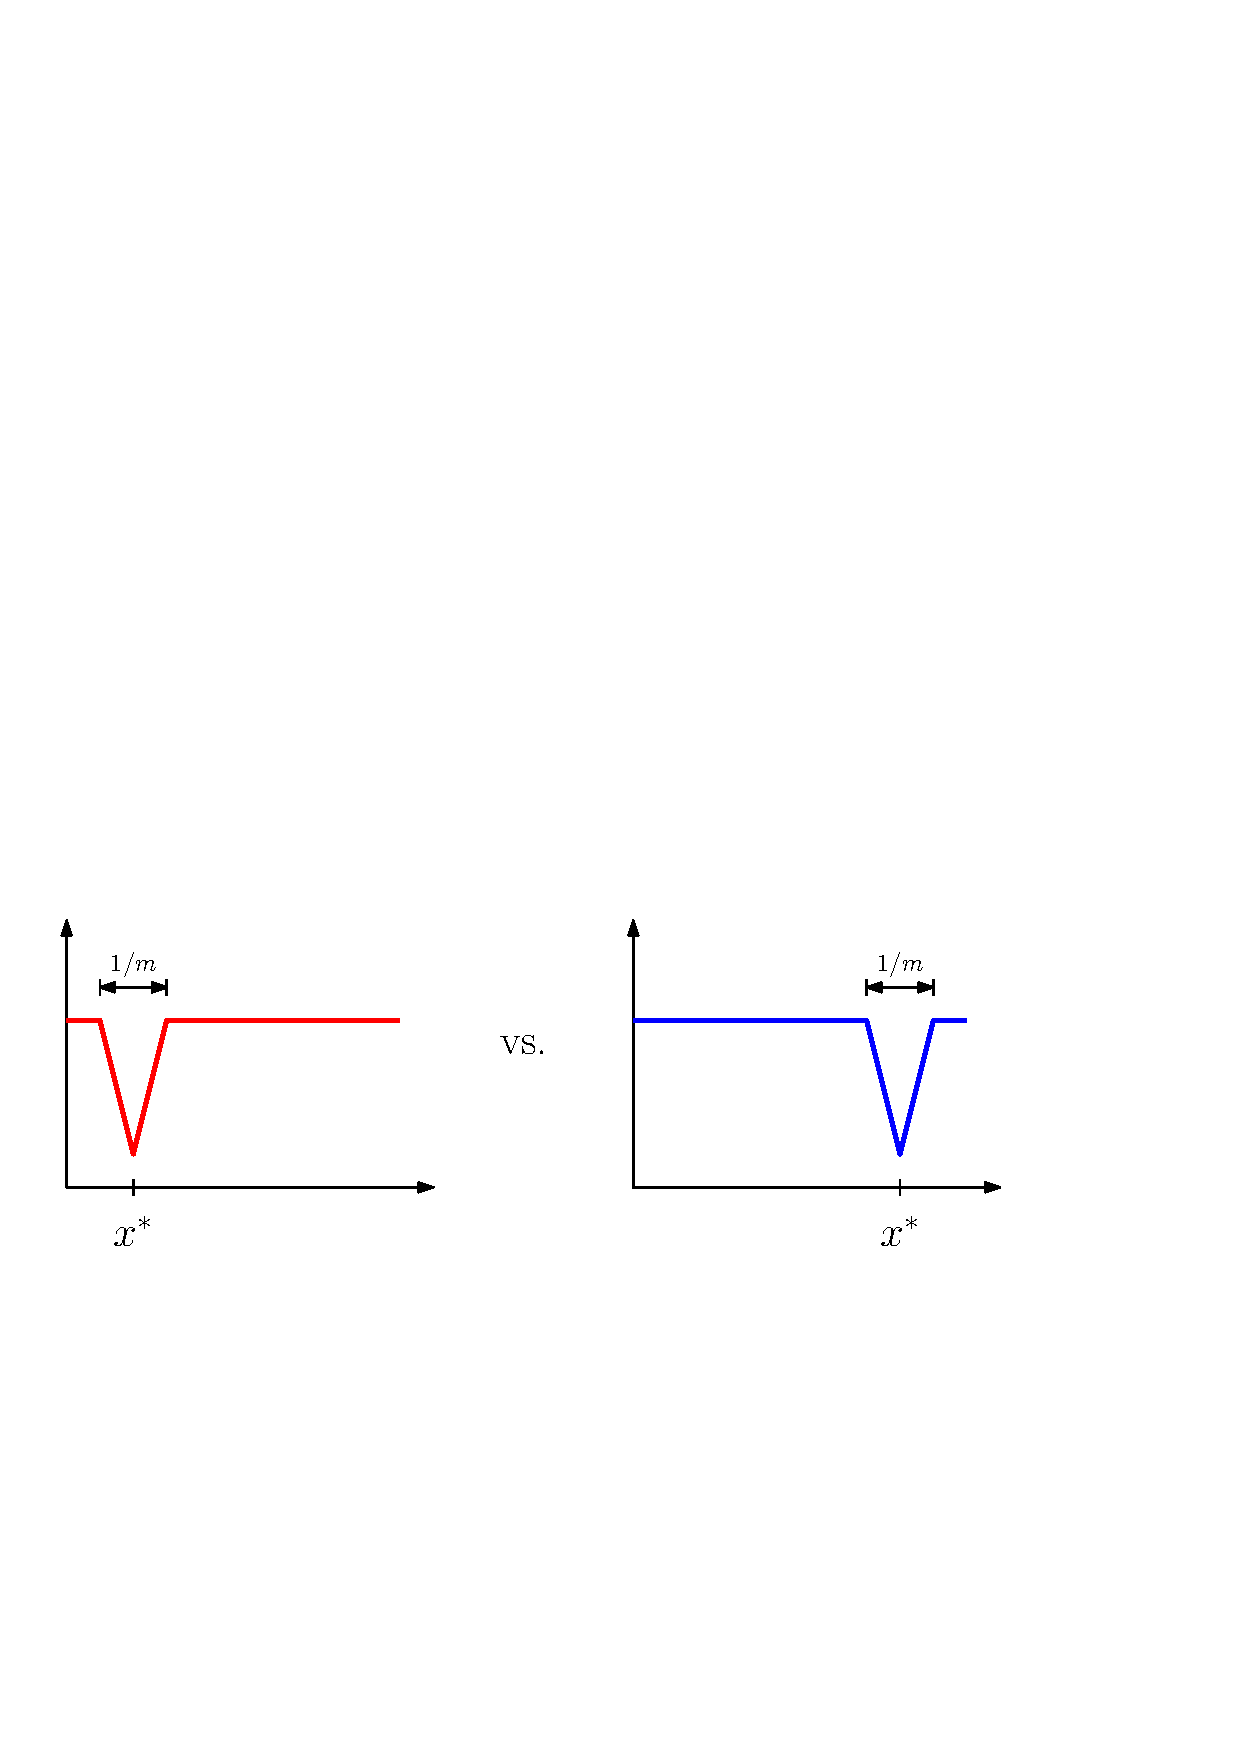
\includegraphics[scale=2]{uniform-conv}
\end{center}

\section*{Open Problems}

\begin{itemize}
\item Is the Hard Margin algorithm consistent in dimension $d \ge 2$?

\item At what rate can $\gamma$, as a function of $m$, decrease so that the Bucketing Algorithm remains consistent?
We know that when $\gamma \in o(\frac{\log m}{m})$ the algorithm is inconsistent. What happens between for rates between $\frac{1}{\sqrt{m}}$
and $\frac{\log m}{m}$.
\end{itemize}

%\nocite{LittlestoneWartmuth1994}
%\nocite{Littlestone1987}
%\nocite{CesaBianchiLugosi2006}

%\bibliographystyle{apalike}
%\bibliography{poster}

\end{multicols}

\end{document}
